%% bare_conf.tex
%% V1.3
%% 2007/01/11
%% by Michael Shell
%% See:
%% http://www.michaelshell.org/
%% for current contact information.
%%
%% This is a skeleton file demonstrating the use of IEEEtran.cls
%% (requires IEEEtran.cls version 1.7 or later) with an IEEE conference paper.
%%
%% Support sites:
%% http://www.michaelshell.org/tex/ieeetran/
%% http://www.ctan.org/tex-archive/macros/latex/contrib/IEEEtran/
%% and
%% http://www.ieee.org/

%%*************************************************************************
%% Legal Notice:
%% This code is offered as-is without any warranty either expressed or
%% implied; without even the implied warranty of MERCHANTABILITY or
%% FITNESS FOR A PARTICULAR PURPOSE!
%% User assumes all risk.
%% In no event shall IEEE or any contributor to this code be liable for
%% any damages or losses, including, but not limited to, incidental,
%% consequential, or any other damages, resulting from the use or misuse
%% of any information contained here.
%%
%% All comments are the opinions of their respective authors and are not
%% necessarily endorsed by the IEEE.
%%
%% This work is distributed under the LaTeX Project Public License (LPPL)
%% ( http://www.latex-project.org/ ) version 1.3, and may be freely used,
%% distributed and modified. A copy of the LPPL, version 1.3, is included
%% in the base LaTeX documentation of all distributions of LaTeX released
%% 2003/12/01 or later.
%% Retain all contribution notices and credits.
%% ** Modified files should be clearly indicated as such, including  **
%% ** renaming them and changing author support contact information. **
%%
%% File list of work: IEEEtran.cls, IEEEtran_HOWTO.pdf, bare_adv.tex,
%%                    bare_conf.tex, bare_jrnl.tex, bare_jrnl_compsoc.tex
%%*************************************************************************

% *** Authors should verify (and, if needed, correct) their LaTeX system  ***
% *** with the testflow diagnostic prior to trusting their LaTeX platform ***
% *** with production work. IEEE's font choices can trigger bugs that do  ***
% *** not appear when using other class files.                            ***
% The testflow support page is at:
% http://www.michaelshell.org/tex/testflow/



% Note that the a4paper option is mainly intended so that authors in
% countries using A4 can easily print to A4 and see how their papers will
% look in print - the typesetting of the document will not typically be
% affected with changes in paper size (but the bottom and side margins will).
% Use the testflow package mentioned above to verify correct handling of
% both paper sizes by the user's LaTeX system.
%
% Also note that the "draftcls" or "draftclsnofoot", not "draft", option
% should be used if it is desired that the figures are to be displayed in
% draft mode.
%
\documentclass[conference]{IEEEtran}
% Add the compsoc option for Computer Society conferences.
%
% If IEEEtran.cls has not been installed into the LaTeX system files,
% manually specify the path to it like:
% \documentclass[conference]{../sty/IEEEtran}





% Some very useful LaTeX packages include:
% (uncomment the ones you want to load)


% *** MISC UTILITY PACKAGES ***
%
%\usepackage{ifpdf}
% Heiko Oberdiek's ifpdf.sty is very useful if you need conditional
% compilation based on whether the output is pdf or dvi.
% usage:
% \ifpdf
%   % pdf code
% \else
%   % dvi code
% \fi
% The latest version of ifpdf.sty can be obtained from:
% http://www.ctan.org/tex-archive/macros/latex/contrib/oberdiek/
% Also, note that IEEEtran.cls V1.7 and later provides a builtin
% \ifCLASSINFOpdf conditional that works the same way.
% When switching from latex to pdflatex and vice-versa, the compiler may
% have to be run twice to clear warning/error messages.






% *** CITATION PACKAGES ***
%
%\usepackage{cite}
% cite.sty was written by Donald Arseneau
% V1.6 and later of IEEEtran pre-defines the format of the cite.sty package
% \cite{} output to follow that of IEEE. Loading the cite package will
% result in citation numbers being automatically sorted and properly
% "compressed/ranged". e.g., [1], [9], [2], [7], [5], [6] without using
% cite.sty will become [1], [2], [5]--[7], [9] using cite.sty. cite.sty's
% \cite will automatically add leading space, if needed. Use cite.sty's
% noadjust option (cite.sty V3.8 and later) if you want to turn this off.
% cite.sty is already installed on most LaTeX systems. Be sure and use
% version 4.0 (2003-05-27) and later if using hyperref.sty. cite.sty does
% not currently provide for hyperlinked citations.
% The latest version can be obtained at:
% http://www.ctan.org/tex-archive/macros/latex/contrib/cite/
% The documentation is contained in the cite.sty file itself.






% *** GRAPHICS RELATED PACKAGES ***
%
\ifCLASSINFOpdf
  \usepackage[pdftex]{graphicx}
  % declare the path(s) where your graphic files are
  % \graphicspath{{../pdf/}{../jpeg/}}
  % and their extensions so you won't have to specify these with
  % every instance of \includegraphics
  % \DeclareGraphicsExtensions{.pdf,.jpeg,.png}
\else
  % or other class option (dvipsone, dvipdf, if not using dvips). graphicx
  % will default to the driver specified in the system graphics.cfg if no
  % driver is specified.
  % \usepackage[dvips]{graphicx}
  % declare the path(s) where your graphic files are
  % \graphicspath{{../eps/}}
  % and their extensions so you won't have to specify these with
  % every instance of \includegraphics
  % \DeclareGraphicsExtensions{.eps}
\fi
% graphicx was written by David Carlisle and Sebastian Rahtz. It is
% required if you want graphics, photos, etc. graphicx.sty is already
% installed on most LaTeX systems. The latest version and documentation can
% be obtained at:
% http://www.ctan.org/tex-archive/macros/latex/required/graphics/
% Another good source of documentation is "Using Imported Graphics in
% LaTeX2e" by Keith Reckdahl which can be found as epslatex.ps or
% epslatex.pdf at: http://www.ctan.org/tex-archive/info/
%
% latex, and pdflatex in dvi mode, support graphics in encapsulated
% postscript (.eps) format. pdflatex in pdf mode supports graphics
% in .pdf, .jpeg, .png and .mps (metapost) formats. Users should ensure
% that all non-photo figures use a vector format (.eps, .pdf, .mps) and
% not a bitmapped formats (.jpeg, .png). IEEE frowns on bitmapped formats
% which can result in "jaggedy"/blurry rendering of lines and letters as
% well as large increases in file sizes.
%
% You can find documentation about the pdfTeX application at:
% http://www.tug.org/applications/pdftex





% *** MATH PACKAGES ***
%
%\usepackage[cmex10]{amsmath}
% A popular package from the American Mathematical Society that provides
% many useful and powerful commands for dealing with mathematics. If using
% it, be sure to load this package with the cmex10 option to ensure that
% only type 1 fonts will utilized at all point sizes. Without this option,
% it is possible that some math symbols, particularly those within
% footnotes, will be rendered in bitmap form which will result in a
% document that can not be IEEE Xplore compliant!
%
% Also, note that the amsmath package sets \interdisplaylinepenalty to 10000
% thus preventing page breaks from occurring within multiline equations. Use:
%\interdisplaylinepenalty=2500
% after loading amsmath to restore such page breaks as IEEEtran.cls normally
% does. amsmath.sty is already installed on most LaTeX systems. The latest
% version and documentation can be obtained at:
% http://www.ctan.org/tex-archive/macros/latex/required/amslatex/math/





% *** SPECIALIZED LIST PACKAGES ***
%
%\usepackage{algorithmic}
% algorithmic.sty was written by Peter Williams and Rogerio Brito.
% This package provides an algorithmic environment fo describing algorithms.
% You can use the algorithmic environment in-text or within a figure
% environment to provide for a floating algorithm. Do NOT use the algorithm
% floating environment provided by algorithm.sty (by the same authors) or
% algorithm2e.sty (by Christophe Fiorio) as IEEE does not use dedicated
% algorithm float types and packages that provide these will not provide
% correct IEEE style captions. The latest version and documentation of
% algorithmic.sty can be obtained at:
% http://www.ctan.org/tex-archive/macros/latex/contrib/algorithms/
% There is also a support site at:
% http://algorithms.berlios.de/index.html
% Also of interest may be the (relatively newer and more customizable)
% algorithmicx.sty package by Szasz Janos:
% http://www.ctan.org/tex-archive/macros/latex/contrib/algorithmicx/




% *** ALIGNMENT PACKAGES ***
%
%\usepackage{array}
% Frank Mittelbach's and David Carlisle's array.sty patches and improves
% the standard LaTeX2e array and tabular environments to provide better
% appearance and additional user controls. As the default LaTeX2e table
% generation code is lacking to the point of almost being broken with
% respect to the quality of the end results, all users are strongly
% advised to use an enhanced (at the very least that provided by array.sty)
% set of table tools. array.sty is already installed on most systems. The
% latest version and documentation can be obtained at:
% http://www.ctan.org/tex-archive/macros/latex/required/tools/


%\usepackage{mdwmath}
%\usepackage{mdwtab}
% Also highly recommended is Mark Wooding's extremely powerful MDW tools,
% especially mdwmath.sty and mdwtab.sty which are used to format equations
% and tables, respectively. The MDWtools set is already installed on most
% LaTeX systems. The lastest version and documentation is available at:
% http://www.ctan.org/tex-archive/macros/latex/contrib/mdwtools/


% IEEEtran contains the IEEEeqnarray family of commands that can be used to
% generate multiline equations as well as matrices, tables, etc., of high
% quality.


%\usepackage{eqparbox}
% Also of notable interest is Scott Pakin's eqparbox package for creating
% (automatically sized) equal width boxes - aka "natural width parboxes".
% Available at:
% http://www.ctan.org/tex-archive/macros/latex/contrib/eqparbox/





% *** SUBFIGURE PACKAGES ***
%\usepackage[tight,footnotesize]{subfigure}
% subfigure.sty was written by Steven Douglas Cochran. This package makes it
% easy to put subfigures in your figures. e.g., "Figure 1a and 1b". For IEEE
% work, it is a good idea to load it with the tight package option to reduce
% the amount of white space around the subfigures. subfigure.sty is already
% installed on most LaTeX systems. The latest version and documentation can
% be obtained at:
% http://www.ctan.org/tex-archive/obsolete/macros/latex/contrib/subfigure/
% subfigure.sty has been superceeded by subfig.sty.



%\usepackage[caption=false]{caption}
%\usepackage[font=footnotesize]{subfig}
% subfig.sty, also written by Steven Douglas Cochran, is the modern
% replacement for subfigure.sty. However, subfig.sty requires and
% automatically loads Axel Sommerfeldt's caption.sty which will override
% IEEEtran.cls handling of captions and this will result in nonIEEE style
% figure/table captions. To prevent this problem, be sure and preload
% caption.sty with its "caption=false" package option. This is will preserve
% IEEEtran.cls handing of captions. Version 1.3 (2005/06/28) and later
% (recommended due to many improvements over 1.2) of subfig.sty supports
% the caption=false option directly:
%\usepackage[caption=false,font=footnotesize]{subfig}
%
% The latest version and documentation can be obtained at:
% http://www.ctan.org/tex-archive/macros/latex/contrib/subfig/
% The latest version and documentation of caption.sty can be obtained at:
% http://www.ctan.org/tex-archive/macros/latex/contrib/caption/




% *** FLOAT PACKAGES ***
%
%\usepackage{fixltx2e}
% fixltx2e, the successor to the earlier fix2col.sty, was written by
% Frank Mittelbach and David Carlisle. This package corrects a few problems
% in the LaTeX2e kernel, the most notable of which is that in current
% LaTeX2e releases, the ordering of single and double column floats is not
% guaranteed to be preserved. Thus, an unpatched LaTeX2e can allow a
% single column figure to be placed prior to an earlier double column
% figure. The latest version and documentation can be found at:
% http://www.ctan.org/tex-archive/macros/latex/base/



%\usepackage{stfloats}
% stfloats.sty was written by Sigitas Tolusis. This package gives LaTeX2e
% the ability to do double column floats at the bottom of the page as well
% as the top. (e.g., "\begin{figure*}[!b]" is not normally possible in
% LaTeX2e). It also provides a command:
%\fnbelowfloat
% to enable the placement of footnotes below bottom floats (the standard
% LaTeX2e kernel puts them above bottom floats). This is an invasive package
% which rewrites many portions of the LaTeX2e float routines. It may not work
% with other packages that modify the LaTeX2e float routines. The latest
% version and documentation can be obtained at:
% http://www.ctan.org/tex-archive/macros/latex/contrib/sttools/
% Documentation is contained in the stfloats.sty comments as well as in the
% presfull.pdf file. Do not use the stfloats baselinefloat ability as IEEE
% does not allow \baselineskip to stretch. Authors submitting work to the
% IEEE should note that IEEE rarely uses double column equations and
% that authors should try to avoid such use. Do not be tempted to use the
% cuted.sty or midfloat.sty packages (also by Sigitas Tolusis) as IEEE does
% not format its papers in such ways.





% *** PDF, URL AND HYPERLINK PACKAGES ***
%
%\usepackage{url}
% url.sty was written by Donald Arseneau. It provides better support for
% handling and breaking URLs. url.sty is already installed on most LaTeX
% systems. The latest version can be obtained at:
% http://www.ctan.org/tex-archive/macros/latex/contrib/misc/
% Read the url.sty source comments for usage information. Basically,
% \url{my_url_here}.





% *** Do not adjust lengths that control margins, column widths, etc. ***
% *** Do not use packages that alter fonts (such as pslatex).         ***
% There should be no need to do such things with IEEEtran.cls V1.6 and later.
% (Unless specifically asked to do so by the journal or conference you plan
% to submit to, of course. )


% correct bad hyphenation here
\hyphenation{op-tical net-works semi-conduc-tor}


\begin{document}
%
% paper title
% can use linebreaks \\ within to get better formatting as desired
\title{Pixel Based Classification Methods in Cassava Brown Streak Disease (CBSD) for Automatic Symptom Measurement}

% author names and affiliations
% use a multiple column layout for up to three different
% affiliations



\author{\IEEEauthorblockN{Joviah Tuhaise}
\IEEEauthorblockA{Department of Computer Science\\
 Makerere University, Uganda\\
Email: tuhaise.joviah@cis.mak.ac.ug}
\and
\IEEEauthorblockN{John A. Quinn}
\IEEEauthorblockA{Department of Computer Science\\
 Makerere University, Uganda\\
Email: jquinn@cit.mak.ac.ug}
\and
\IEEEauthorblockN{Ernest Mwebaze}
\IEEEauthorblockA{Department of Computer Science\\
Makerere University, Uganda\\
Email: emwebaze@cit.mak.ac.ug}
}



% conference papers do not typically use \thanks and this command
% is locked out in conference mode. If really needed, such as for
% the acknowledgment of grants, issue a \IEEEoverridecommandlockouts
% after \documentclass

% for over three affiliations, or if they all won't fit within the width
% of the page, use this alternative format:
%
%\author{\IEEEauthorblockN{Michael Shell\IEEEauthorrefmark{1},
%Homer Simpson\IEEEauthorrefmark{2},
%James Kirk\IEEEauthorrefmark{3},
%Montgomery Scott\IEEEauthorrefmark{3} and
%Eldon Tyrell\IEEEauthorrefmark{4}}
%\IEEEauthorblockA{\IEEEauthorrefmark{1}School of Electrical and Computer Engineering\\
%Georgia Institute of Technology,
%Atlanta, Georgia 30332--0250\\ Email: see http://www.michaelshell.org/contact.html}
%\IEEEauthorblockA{\IEEEauthorrefmark{2}Twentieth Century Fox, Springfield, USA\\
%Email: homer@thesimpsons.com}
%\IEEEauthorblockA{\IEEEauthorrefmark{3}Starfleet Academy, San Francisco, California 96678-2391\\
%Telephone: (800) 555--1212, Fax: (888) 555--1212}
%\IEEEauthorblockA{\IEEEauthorrefmark{4}Tyrell Inc., 123 Replicant Street, Los Angeles, California 90210--4321}}

% use for special paper notices
%\IEEEspecialpapernotice{(Invited Paper)}

% make the title area
\maketitle


\begin{abstract}
%\boldmath
The rapid geographical expansion of the Cassava Brown Streak Disease (CBSD) pandemic has devastated cassava crops in East and Central Africa. To monitor CBSD, surveyors deal with single fields of plants at a time. A score of severity of disease is visually assigned to the plant based on the percentage of necrotised root of the cross-sections cuttings of the root examined. This method has problems with operator variability. This study investigates various computer vision techniques which leads to the development of a system whose feasibility is later assessed and it involves five stages. In stage one, using mobile deployment, images were acquired. Stage two involves use of different techniques to obtain an annotated data set where each pixel is later classified as healthy or necrotised in stage three. The classifiers used in this study were: Nearest Neighbors, Decision Tree, Random Forest, Naive Bayes and Support Vector Machine classifier (Linear SVM). In stage four, the performance of these classifiers was evaluated based on the Area Under the Curve (AUC) analysis and accuracy results which evaluated how good the classifiers performed when distinguishing necrotised pixels from healthy pixels, Mean Absolute Error (MAE) and $R^{2}$ score, the coefficient of determination evaluated how good the classifiers performed in the overall prediction of the percentage of necrotisation in the root. With the $R^{2}$ score of 0.789, Nearest Neighbors classifier performed better than the other classifiers and thus it was recommended as the best method assign a score of necrosis to the diseased cross-section cuttings of the cassava root. And lastly, to assess whether a standardised automated system for measuring root necrosis in cassava is feasible, two performance measures were used  i.e. linear least squares fitting and a confusion matrix.
\end{abstract}
% IEEEtran.cls defaults to using nonbold math in the Abstract.
% This preserves the distinction between vectors and scalars. However,
% if the conference you are submitting to favors bold math in the abstract,
% then you can use LaTeX's standard command \boldmath at the very start
% of the abstract to achieve this. Many IEEE journals/conferences frown on
% math in the abstract anyway.

% no keywords




% For peer review papers, you can put extra information on the cover
% page as needed:
% \ifCLASSOPTIONpeerreview
% \begin{center} \bfseries EDICS Category: 3-BBND \end{center}
% \fi
%
% For peerreview papers, this IEEEtran command inserts a page break and
% creates the second title. It will be ignored for other modes.
\IEEEpeerreviewmaketitle



\section{Introduction}
% no \IEEEPARstart
Cassava (Manihot esculenta) is an extremely important crop in Africa: $200$ million people in the continent depend on it. In Sub-Sahara Africa, cassava can represent up to 60\% of the daily calorie intake, and is largely consumed locally. Cassava requires a little farming and inputs, and therefore cassava plants usually survive where other crops cannot. This generates cash income for a large number of households as compared to other food staples \cite{nassar2007cassava}. Cassava grows in moderately poor soils with limited labor requirements and it tolerates drought thus cassava is a significant food security crop, mainly in drought-stricken areas \cite{chavez2005variation}.\\ \\ The leading diseases affecting cassava in these areas are CBSD and Cassava Mosaic Disease (CMD). CBSD is a risk to food security, because the severity of root damage caused by the disease escalates the longer it stays in the field. CBSD, which is caused by a virus, was at first confined to coastal, low altitude areas in East Africa, but since the mid-2000s the disease has spread speedily, affecting Tanzania, Uganda, Kenya, Rwanda and Burundi. The disease has at present infected around $80\%$ of crops in Uganda and around $20\%$ of crops in Rwanda and Burundi \cite{cass}. CBSD is a more significant cause of crop loss in these regions than was earlier believed \cite{ntawuruhunga2007new} since the disease causes both quantitative and qualitative decrease in total root yield by rotting of roots thus making them unmarketable and unpalatable. For cassava plants infected with CBSD, the major part affected is the tuber/root of the plant. To monitor CBSD, surveyors deal with single fields of plants at a time. When out in the field, normally they dig up a set of plants in selected gardens and examine five cross-section cuttings of the root. A score of severity of disease is allocated to the plant based on the average percentage of necrotised root of all five cross-sections examined. However, visual assessment of the symptoms to determine the score of severity of disease of a root by an expert may differ from the score of severity by another thus rendering this method ineffective. To quantify the problem of operator variability, we asked two experts to assign scores of severity of disease to the same cassava cross-section cutting of the root, the results were obtained and the level of disagreement was obtained. This paper provides the innovation to overcome this challenge. We present computer vision techniques for using camera-enabled mobile devices to automatically assign a score of severity of necrosis directly, allowing confidence on survey workers with lower levels of training, and thus reducing survey costs. Precisely, given expert-annotated single images of infected cassava tubers, we demonstrate classification based on pixel information.\\ \\ In the developing countries, one of the reasons why crop disease surveys are more likely to be under resourced is shortage of expert surveyors. Dependable automatic methods for performing surveys hence would offer the possibility of extending the scope of CBSD disease monitoring. The prevalence of mobile computing devices offers a realistic alternative to paper-based data collecting and the possibility of survey by non-expert workers who submit images of crops that are then automatically classified

\subsection{Related work}
According to Mahlein et al. \cite{Mahlein201321}, \ac{SVIs} have been shown to be useful for an indirect detection of plant diseases. Nevertheless, these indices have not been evaluated to detect or to differentiate between plant diseases on crop plants. The study developed specific \ac{SDIs} for the detection of diseases in crops. Sugar beet plants and the three leaf diseases Cercospora leaf spot, sugar beet rust and powdery mildew were used as sample diseases. Hyperspectral signatures of healthy and diseased sugar beet leaves were assessed with a non-imaging spectroradiometer at different developing stages and disease severities of pathogens. To develop hyperspectral indices for the detection of sugar beet diseases the best weighted combination of a single wavelength and a normalised wavelength difference was thoroughly searched testing all potential groupings. The optimised disease indices were tested for their ability to detect and to classify healthy and diseased sugar beet leaves. With a high accuracy and sensitivity healthy sugar beet leaves and leaves, infected with Cercospora leaf spot, sugar beet rust and powdery mildew were classified. Spectral disease indices were also successfully applied on hyperspectral imaging data and on non-imaging data from a sugar beet field.\\ \\ Smith and Camargo \cite{Smith2009image} developed an image-processing based algorithm to automatically identify plant disease visual symptoms. The study described an image-processing based method that identifies the visual symptoms of plant diseases by analysis of colored images. Results showed that the developed algorithm was able to identify a diseased region even when that region was represented by a wide range of intensities.\\ \\ A hybrid intelligent system from color imagery for grape leaf disease detection was suggested by \cite{meunkaewjinda2008grape}. The system consisted of three core parts i.e. grape leaf color segmentation, grape leaf disease segmentation and classification of diseases. The system was able to classify the image of grape leaf into three classes which are; scab disease, rust disease and no disease.\\ \\ Smith and Camargo \cite{camargo2009image} performed an image pattern classification for the identification of disease causing agents in plants. A machine vision system for the classification of the visual symptoms of plant diseases was implemented by analysis of colored images. A set of image features was extracted from each diseased region. Feature selection was then performed to identify which of these provided most information about the image domain. An SVM was used as a learning machine and cross-validation was the discrimination method used to identify the best classification model.



% You must have at least 2 lines in the paragraph with the drop letter
% (should never be an issue)

%\hfill mds

%\hfill August 30, 2014

\subsection{Methods}
\subsubsection{Image Acquisition}
Image samples of cross sectional cut cassava tubers placed on a plain board were captured from Namulonge Crops resources Research Institute, Uganda. $15$ root discs from the same genotype of cassava were cross sectionally cut, placed on a plain board and captured with a standard digital camera.

\begin{figure}[t!]
\centering
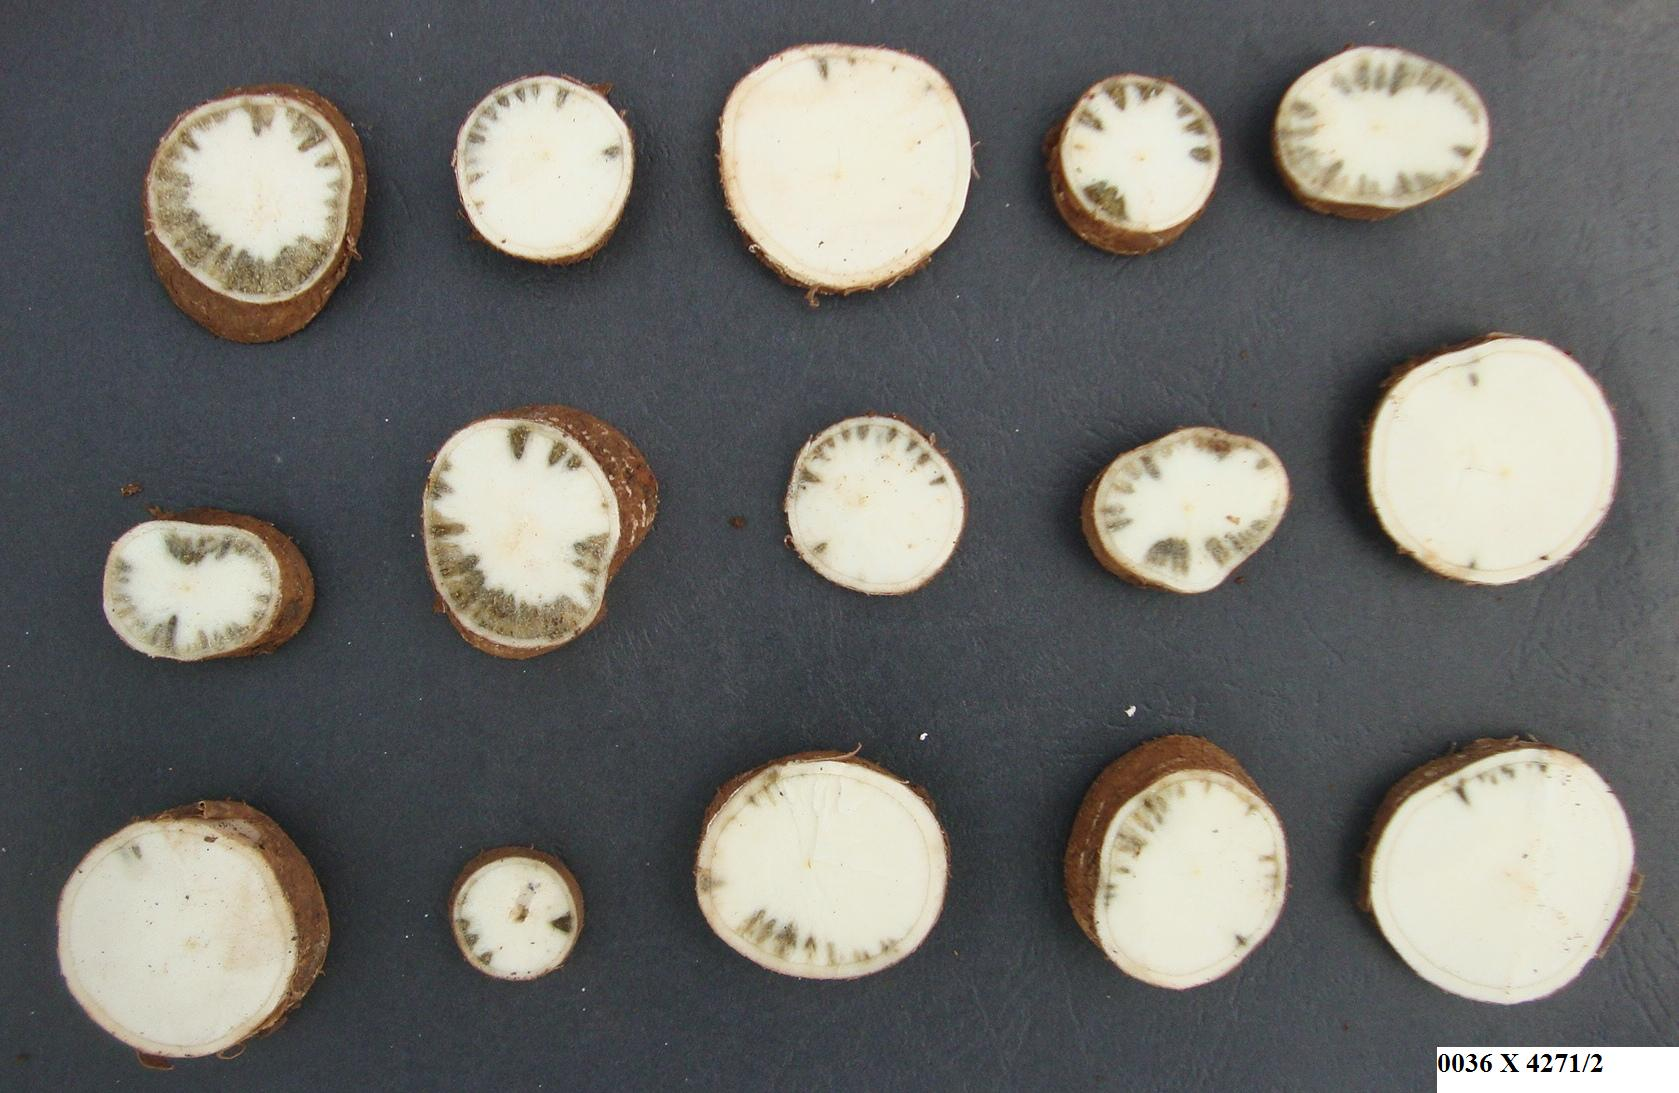
\includegraphics[scale=0.15]{images/cassava1.jpg}
\caption{Image sample as captured by camera}
\label{fig:figure3}
\end{figure}


\subsubsection{Image Segmentation}
In this study, images were cropped manually using a cropping tool. However, cropped images had a white background and working with the whole image also brings inaccurate results too. To eliminate the white back ground, only non-pure white pixels in the image were extracted automatically, Samples of the resulting cropped image and binary image are shown in Figure \ref{fig:figure4} and Figure \ref{fig:figure5} respectively.

\begin{figure}[t!]
\centering
\begin{minipage}[b]{0.3\linewidth}
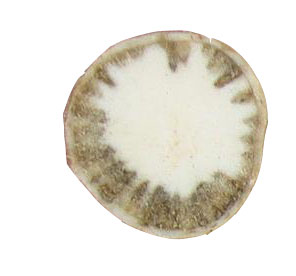
\includegraphics[width=\textwidth]{images/cropped.jpg}
\caption{Cropped image}
\label{fig:figure4}
\end{minipage}
\hspace{0.5cm}
\begin{minipage}[b]{0.3\linewidth}

\includegraphics[width=\textwidth]{images/croppedbinary.jpg}
\caption{Binary image}
\label{fig:figure5}
\end{minipage}
\end{figure}

A threshold was applied separately to each cropped root image so as to obtain its respective binary image as shown above. Coordinates of the non-pure white pixels were obtained. Using these coordinates, from the respective binary image, each pixel was labeled healthy or necrotised.

\subsubsection{Ground Truth Data}
Image pixel data was extracted from the original image and its corresponding binary image. From the original image, the $RGB$ pixel data with the corresponding location coordinates,$(i,j)$ were extracted as shown in Table \ref{tbl:rgbpix}

\begin{table}[t!]
\renewcommand{\arraystretch}{1.3}
 \caption{Sample pixels under $RGB$ color space }
\centering
\begin{tabular}{|l|l|l|l|l|}
      \hline
      r & g & b & i & j \\ \hline
      254 & 254  & 254  & 56 & 106 \\ \hline
      254 & 254  & 254  & 56 & 107 \\  \hline
      254 & 254  & 254  & 56 & 108 \\  \hline
      247 & 253  & 249  & 56 & 112 \\  \hline
      254 & 254  & 254  & 57 & 109 \\ \hline
      121 & 95  & 60  & 216 & 209 \\ \hline
      252 & 252  & 252  & 57 & 114 \\ \hline
      95 & 72  & 40  & 216 & 211\\ \hline
    \end{tabular}}
    \label{tbl:rgbpix}
\end{table}


\subsubsection{Evaluation of the Classifier Performance}
To evaluate classifier performance, four performance measures were implemented, i.e., Receiver Operating Characteristic (ROC), AUC and predictive accuracy score, which evaluated how good the classifiers performed when distinguishing necrotised pixels from healthy pixels. MAE and $R^{2}$ score, the coefficient of determination evaluated how good the classifiers performed in the overall prediction of the percentage of necrotisation in the root.

\subsubsection{Receiver Operating Characteristics}
To choose the best performing classifier, results of AUC and accuracy were obtained. In this section the results for both methods will be presented. A ROC graph is a technique for visualising, organising and selecting classifiers based on their performance. Given a classifier and an instance, there are four possible outcomes, i.e., true positive $(TP)$, false negative $(FN)$, true negative $(TN)$ and false positive $(FP)$ \cite{fawcett2006introduction}. Table \ref{tbl:img1} shows the results for AUC obtained for the different classifiers for the RGB color space. If a classifier yields a 1.0, then it is a perfect test. 0.9 to 0.99 is an excellent test, 0.8 to 0.89 is a good test, 0.7 to 0.79 is a fair test, 0.6 to 0.69 is a poor test, 0.5 to 0.59 is a failed test and below 0.5 the classifier is negatively correlated with the target.
\begin{table}[t!]
\renewcommand{\arraystretch}{1.3}
\caption{AUC of classifiers for $RGB$ color space }
\centering
    \begin{tabular}{|l|l|l|l|l|}
      \hline
      Sample Image &Image1 &Image2 & Image3 & Image4 \\ \hline

      Naive Bayes & 0.96  & 0.96 & 0.96 & 0.96 \\    \hline
      Linear SVM & 0.97  & 0.96 & 0.97 & 0.97 \\      \hline
      Decision Tree & 0.96  & 0.96 & 0.97 & 0.96 \\      \hline
      Nearest Neighbors & 0.96  & 0.96 & 0.96 & 0.96 \\      \hline
      Random Forests & 0.97  & 0.97& 0.97 & 0.97 \\      \hline
     \end{tabular}
    \label{tbl:img1}
\end{table}

\subsubsection{Predictive Accuracy Score}
Classifiers were also assessed based on the predictive accuracy score with cross-validation. The accuracy of the test approximates how effective the algorithm is by showing the probability of the true value of the class label; summing it all up, it evaluates the overall effectiveness of the algorithm \cite{sokolova2006beyond}. The higher the probability, the higher the predictive accuracy score. Four sample images were used to determine the probabilities as shown in Table \ref{tbl:img11}.



\begin{table}[t!]
\renewcommand{\arraystretch}{1.3}
\caption{Accuracy score of classifiers for $RGB$ color space }
\centering
    \begin{tabular}{|l|l|l|l|l|}
      \hline
      Sample Image &Image1 &Image2 & Image3 & Image4 \\ \hline

      Naive Bayes & 0.90  & 0.89 & 0.90 & 0.89 \\    \hline
      Linear SVM &  0.92 & 0.91 & 0.91  & 0.92 \\      \hline
      Decision Tree &  0.92 &  0.92 & 0.92 & 0.92 \\      \hline
      Nearest Neighbors &  0.92 &  0.92 & 0.92 & 0.92 \\      \hline
      Random Forests &  0.92 &  0.92 & 0.92 & 0.92 \\      \hline
    \end{tabular}

    \label{tbl:img11}
\end{table}


\subsubsection{Mean Absolute Error (MAE)}

The (MAE) was used to measure how close predictions of the overall percentage of necrotisation of a root were to the actual percentage of necrotisation of the root. The \ac{MAE} estimated over $n_{\text{samples}}$ is defined as is defined as;

\begin{equation}\label{eqn13}
    \text{MAE}(y, \hat{y}) = \frac{1}{n_{\text{samples}}} \sum_{i=1}^{n_{\text{samples}}} \left| y_{i} - \hat{y}_{i} \right|.
\end{equation}

\noindent where $\hat{y}_{i}$ is the predicted value of the $i$-th sample and $y_{i}$ is the corresponding true value.

\noindent The results for (MAE) for the different classifiers are shown in Table \ref{tbl:mae}.

\begin{table}[t!]
\renewcommand{\arraystretch}{1.3}
\caption{Mean Absolute Error for the different classifiers }\label{tbl:mae}
\centering

    \begin{tabular}{|l|l|}
    \hline
      Classifier & Mean Absolute Error  \\   \hline
      Naive Bayes & 0.049044    \\ \hline
      Linear SVM & 0.059612  \\    \hline
      Decision Tree &  0.052787  \\   \hline
      Nearest Neighbors & 0.049044   \\    \hline
      Random Forest & 0.053079   \\    \hline
    \end{tabular}

\end{table}

\noindent Naive Bayes classifier and Nearest Neighbors classifier had the lowest (MAE) of \emph{0.049044} while the other classifiers had a slightly higher MAE. This meant that Naive Bayes classifier and Nearest Neighbors classifier were more reliable models compared to the other classifiers.

\subsubsection{$R^{2}$ Score, the Coefficient of Determination}

The $R^{2}$ score, the coefficient of determination was calculated and this provided results on how well the overall percentage of necrotisation is predicted by the model. If $\hat{y}_{i}$ is the predicted value of the $i$-th sample and $y_{i}$ is the corresponding true value, then the score $R^{2}$ estimated over $n_{\text{samples}}$ is defined as,

\begin{equation}\label{eqn9}
    R^2(y, \hat{y}) = 1 - \frac{\sum_{i=1}^{n_{\text{samples}}} (y_{i} - \hat{y}_{i})^{2}}{\sum_{i=1}^{n_\text{samples}} (y_{i} - \bar{y})^{2}}
\end{equation}

\noindent where $\bar{y} =  \frac{1}{n_{\text{samples}}} \sum_{i=1}^{n_{\text{samples}}} y_{i}$.

\noindent The results for $R^{2}$ score for the different classifiers are shown in Table \ref{tbl:r2} below.


\begin{table}[Htbp]
\renewcommand{\arraystretch}{1.3}
\caption{$R^{2}$ score for the different classifiers }\label{tbl:r2}
\centering
    \begin{tabular}{|l|l|}
    \hline
      Classifier & $R^{2}$ score   \\ \hline
      Naive Bayes &   0.69107  \\
      \hline
      Linear SVM &  0.60568 \\
      \hline
      Decision Tree & 0.68858   \\
      \hline
      Nearest Neighbors &  0.78955  \\
      \hline
      Random Forest & 0.66258   \\    \hline
    \end{tabular}

\end{table}


\noindent Based on the results, comparing the classifiers used, the Nearest Neighbors classifier had the highest result of the {$R^{2}$ score of \emph{0.78955}. This means that \emph{79\% }of the total variation in Actual Percentage Necrosis is determined by the linear relationship between Nearest Neighbors Percentage Necrosis and the Actual Percentage Necrosis. Because of the highest result of the {$R^{2}$ score compared to other classifiers, Nearest Neighbors classifier proved to be the more reliable the model.

\subsection{Assessing Feasibility of the System}
The score of necrosis that was visually assigned by an expert from Namulonge Crops resources Research Institute, the predicted score of necrosis and the actual score of necrosis for the sample images was compared. To assess the feasibility of the model designed, two performance measures were used i.e. Linear least squares fitting and a confusion matrix.


\subsubsection{Confusion Matrix}
To assess operator variability, by comparing two sets of predictions of two different surveyors, a confusion matrix was used to determine how these predictions differed. The results are shown in Figure \ref{fig:CONM} and Table \ref{tbl:CM}:



\begin{figure}[t!]
\centering
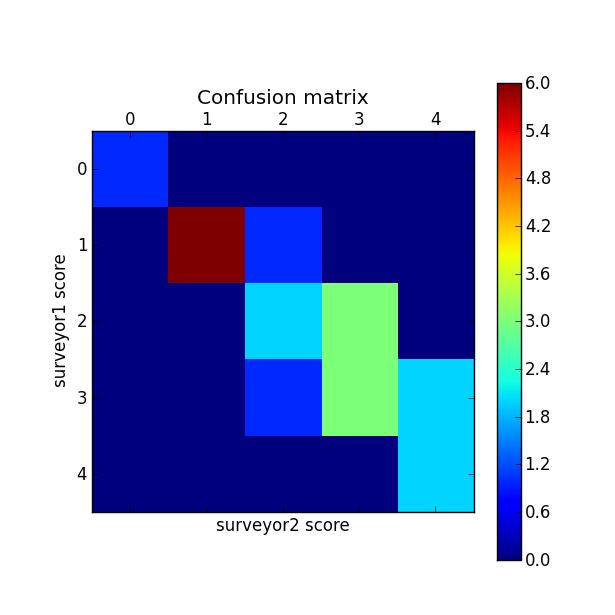
\includegraphics[scale=0.2]{images/confusionmatrix.jpg}
\caption{Surveyor Score comparison for the two surveyors }
\label{fig:CONM}
\end{figure}

\begin{table}[t!]
\renewcommand{\arraystretch}{1.3}
\caption{Surveyor Score confusion matrix }
\centering
    \begin{tabular}{|l|
    lllll|}
    \hline
     Scores&1 & 2  & 3 & 4 & 5  \\    \hline
     1& 1 & 0  & 0 & 0 & 0  \\
     2& 0 & 6  & 1 & 0 & 0  \\
     3& 0 & 0  & 2 & 3  & 0    \\
     4& 0 & 0  & 1 & 3  & 2 \\
     5& 0 & 0  & 0 & 0  & 2 \\ \hline
    \end{tabular}

    \label{tbl:CM}
\end{table}}


Referring to Table \ref{tbl:CM}:
\begin{itemize}
  \item The \emph{rows} correspond to the score results as assigned by Surveyor2.
  \item The \emph{columns} correspond to the score results as assigned by Surveyor1.
  \item The \emph{diagonal elements} in the matrix represent the number of same score results that both surveyors assigned to the same image.
  \item The \emph{off-diagonal elements} represent the score results that were assigned differently by both surveyors to the same images.
      \begin{itemize}
        \item Off-diagonal row elements represent Surveyor1's score results that differed from Surveyor2's score results. E.g. In the second row, one image was assigned a score \emph{2} by Surveyor1 and Surveyor2 assigned the same image a score of \emph{3}.
        \item Off-diagonal column elements represent Surveyor2's score results that differed from Surveyor1's score results. E.g. In the fourth column, three images were assigned a score of \emph{4} by Surveyor2 and Surveyor1 assigned the same image a score of \emph{3}.
      \end{itemize}
\end{itemize}


 Based on the outcome of the confusion matrix, it is seen that different scores are assigned to the same image by two different surveyors. This shows how this method has problems with operator variability and therefore an automated system is a more feasible solution as compared to the surveyor visual assignment method.

\subsubsection{Linear Least Squares Fitting}
 Linear least squares fitting is a statistical method used to determine a line of best fit by minimising the sum of squares created by a mathematical function and a "square" is determined by squaring the distance between a data point and the fitted line. In this case, the goal was to ascertain the relationship between different pairs of variables. And these were:

\begin{itemize}
  \item Surveyor1 \& 2 Score and Predicted necrosis Percentage.
  \item Actual necrosis Percentage and Predicted necrosis Percentage.
  \item Actual necrosis Percentage and Surveyor1 \& Surveyor2 Score.
\end{itemize}


\subsubsection{Actual Necrosis Percentage}
To calculate the actual percentage of necrosis of a given test image, the binary pixel labels, i.e $(1,0)$ were used. From Equation \ref{act},

\begin{equation}\label{act}

     Actual\,\%\, of\, Necrosis = \left(\frac{\sum (pixels \,labeled \,(0))}{\sum (pixels\, labeled\, (0,1))}\right)\,\times

     \,100
\end{equation}



Linear least squares fitting graphs were plotted as shown in Figures \ref{fig:Relatio1}, \ref{fig:Relatio2} and \ref{fig:Relatio3}.

\begin{figure}[t!]
\centering
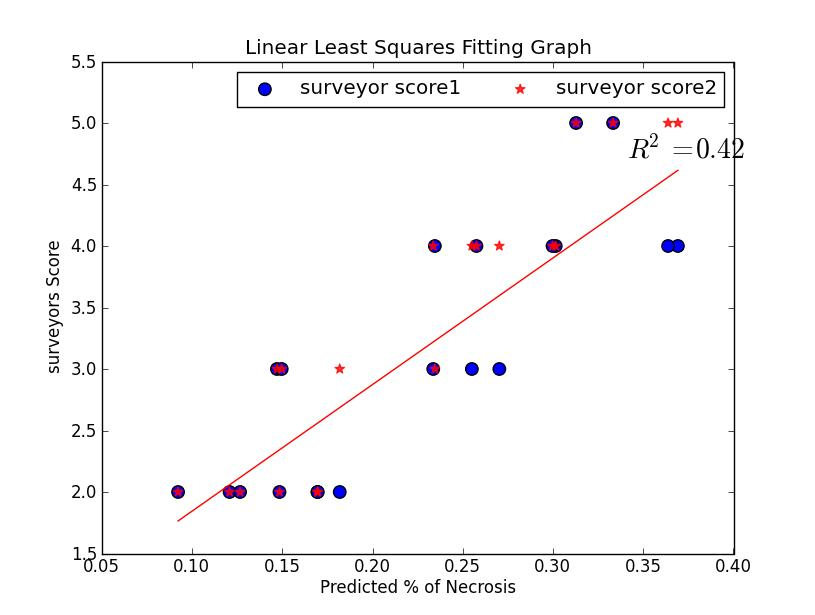
\includegraphics[scale=0.25]{images/Suveyor_predicted.jpg}
\caption{Surveyor Score and Predicted necrosis Percentage}
\label{fig:Relatio1}
\end{figure}

\begin{figure}[t!]
\centering
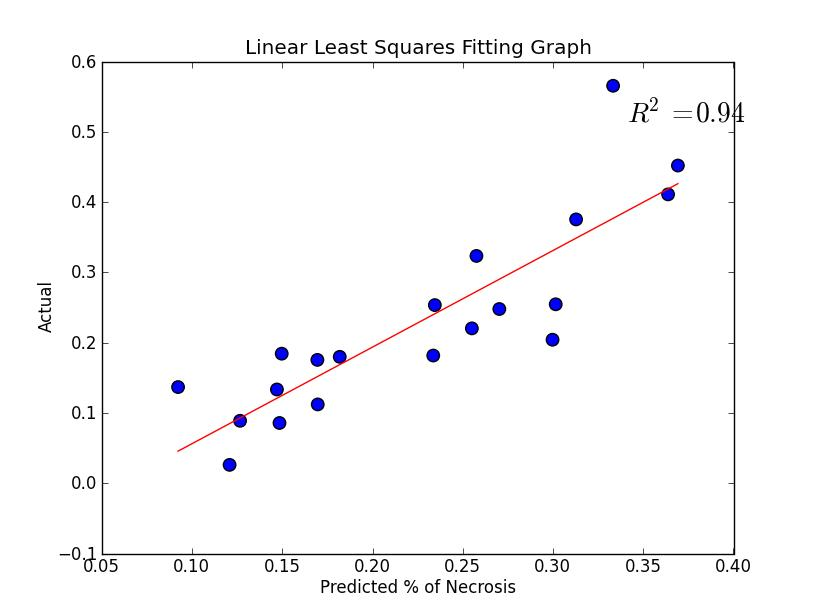
\includegraphics[scale=0.25]{images/Actual_Predicted.jpg}
\caption{Actual necrosis Percentage and Predicted necrosis Percentage}
\label{fig:Relatio2}
\end{figure}

\begin{figure}[t!]
\centering
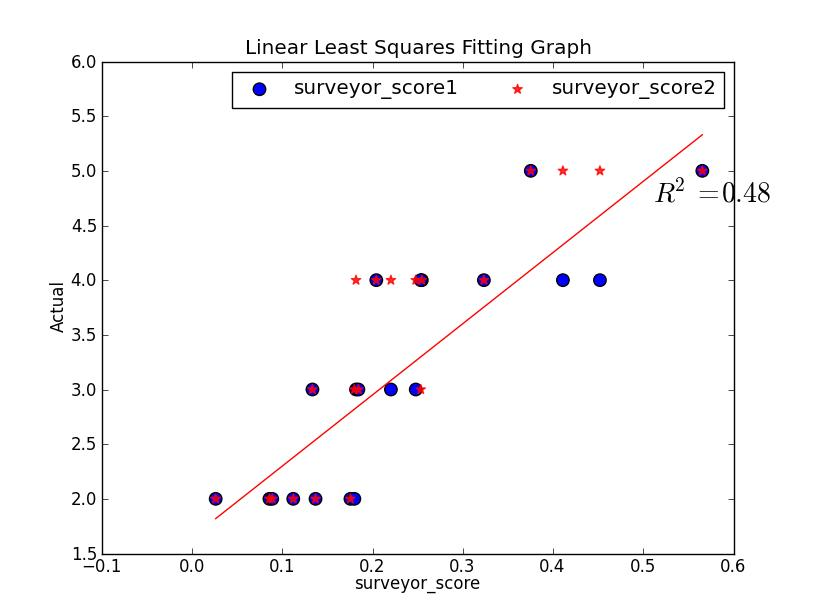
\includegraphics[scale=0.25]{images/Actual_surveyor.jpg}
\caption{ Actual necrosis Percentage and Surveyor Score }
\label{fig:Relatio3}
\end{figure}


\begin{table}[t!]
\renewcommand{\arraystretch}{1.3}
\caption{$R^{2}$ score for the different relationships }

    \begin{tabular}{|l|l|}
    \hline
      Relationship & $R^{2}$ score  \\    \hline
      Surveyor Score and Predicted necrosis Percentage & 0.42  \\\hline
      Actual necrosis Percentage and Predicted necrosis Percentage & 0.94  \\\hline
      Actual necrosis Percentage and Surveyor Score & 0.48  \\ \hline
    \end{tabular}


    \label{tbl:fitting}
\end{table}}

$R^{2}$ is a measure of how close the data are to the line and the higher the $R^{2}$, the better the model fits the data. Based on the results in Table \ref{tbl:fitting}, the $R^{2}$ score of actual necrosis percentage and predicted necrosis percentage is very high compared to actual necrosis percentage and surveyor score. This means from the results in Table \ref{tbl:fitting}, the model designed will predict the overall percentage of necrosis of a root well.

Based on the results of the confusion matrix and the $R^{2}$ score after the linear squares fitting, it is seen how an automated system is a more feasible solution as compared to the method of surveyor visual score assignment. From the confusion matrix, the difference in scores by the surveyors to the same image shows how the surveyor visual score assignment has problems with operator variability. From the results of the $R^{2}$ score of actual necrosis percentage and predicted necrosis percentage being \emph{0.94} and the highest as compared to actual necrosis percentage and surveyor score with an $R^{2}$ score of \emph{0.48},  an automated score assignment to the necrotised root is a more feasible solution as compared to the method of surveyor visual score assignment.



% An example of a floating figure using the graphicx package.
% Note that \label must occur AFTER (or within) \caption.
% For figures, \caption should occur after the \includegraphics.
% Note that IEEEtran v1.7 and later has special internal code that
% is designed to preserve the operation of \label within \caption
% even when the captionsoff option is in effect. However, because
% of issues like this, it may be the safest practice to put all your
% \label just after \caption rather than within \caption{}.
%
% Reminder: the "draftcls" or "draftclsnofoot", not "draft", class
% option should be used if it is desired that the figures are to be
% displayed while in draft mode.
%
%\begin{figure}[!t]
%\centering
%\includegraphics[width=2.5in]{myfigure}
% where an .eps filename suffix will be assumed under latex,
% and a .pdf suffix will be assumed for pdflatex; or what has been declared
% via \DeclareGraphicsExtensions.
%\caption{Simulation Results}
%\label{fig_sim}
%\end{figure}

% Note that IEEE typically puts floats only at the top, even when this
% results in a large percentage of a column being occupied by floats.


% An example of a double column floating figure using two subfigures.
% (The subfig.sty package must be loaded for this to work.)
% The subfigure \label commands are set within each subfloat command, the
% \label for the overall figure must come after \caption.
% \hfil must be used as a separator to get equal spacing.
% The subfigure.sty package works much the same way, except \subfigure is
% used instead of \subfloat.
%
%\begin{figure*}[!t]
%\centerline{\subfloat[Case I]\includegraphics[width=2.5in]{subfigcase1}%
%\label{fig_first_case}}
%\hfil
%\subfloat[Case II]{\includegraphics[width=2.5in]{subfigcase2}%
%\label{fig_second_case}}}
%\caption{Simulation results}
%\label{fig_sim}
%\end{figure*}
%
% Note that often IEEE papers with subfigures do not employ subfigure
% captions (using the optional argument to \subfloat), but instead will
% reference/describe all of them (a), (b), etc., within the main caption.


% An example of a floating table. Note that, for IEEE style tables, the
% \caption command should come BEFORE the table. Table text will default to
% \footnotesize as IEEE normally uses this smaller font for tables.
% The \label must come after \caption as always.
%
%\begin{table}[!t]
%% increase table row spacing, adjust to taste
%\renewcommand{\arraystretch}{1.3}
% if using array.sty, it might be a good idea to tweak the value of
% \extrarowheight as needed to properly center the text within the cells
%\caption{An Example of a Table}
%\label{table_example}
%\centering
%% Some packages, such as MDW tools, offer better commands for making tables
%% than the plain LaTeX2e tabular which is used here.
%\begin{tabular}{|c||c|}
%\hline
%One & Two\\
%\hline
%Three & Four\\
%\hline
%\end{tabular}
%\end{table}


% Note that IEEE does not put floats in the very first column - or typically
% anywhere on the first page for that matter. Also, in-text middle ("here")
% positioning is not used. Most IEEE journals/conferences use top floats
% exclusively. Note that, LaTeX2e, unlike IEEE journals/conferences, places
% footnotes above bottom floats. This can be corrected via the \fnbelowfloat
% command of the stfloats package.

\section{Conclusion}
The research has proved that an automatic symptom measurement system specifically one that assigns a score to a necrotised cassava tuber infected with CBSD is a more feasible solution as compared to the surveyor visual score assignment method and if used, would avert the challenge of inconsistent data collection by surveyors and would speed up the process of developing new cassava varieties that are resistant to CBSD. It has been shown how different classification techniques have been applied to automatically assign the score to the cassava tuber. Five classifiers were tested to get results; all classifiers performed well though some performed better than others. Nearest Neighbors classifier and Naive Bayes classifier had the lowest MAE, however Nearest Neighbors classifier had the highest result of the {$R^{2}$ score and based on that, it was proved to be the more reliable the model as compared to the other four classifiers. The model was assessed and the results proved that it was a more feasible solution as compared to the method of visual assignment of the score of necrosis. In the assessment of the feasibility of the model, based on the results of the confusion matrix and the $R^{2}$ score after the linear squares fitting, it was shown how an automated system is a more feasible solution as compared to the method of surveyor visual score assignment. From the confusion matrix, the difference in scores by the surveyors to the same image showed how the surveyor visual score assignment has problems with operator variability. From the results of the $R^{2}$ score of actual necrosis percentage and predicted necrosis percentage being the highest as compared to actual necrosis percentage and surveyor score with an $R^{2}$ score, it was demonstrated that an automated score assignment to the necrotised root is a more feasible solution as compared to the method of surveyor visual score assignment.\\ \\ The work can be incorporated in to a mobile version. This can be done by using Open Data Kit (ODK) which is a is an open source suite of tools that enables data collection on mobile phones and data submissions to a central server. This could then improve on the monitoring of cassava brown streak disease by providing real-time information because not only experts but volunteers or farmers can take the images and then they can be uploaded on to a server at the research institute where they can be processed. Furthermore, it could improve on the prediction and optimisation of plant protection measures since there is consistence of results because everyone uses the same tool. Two experts can give two different scores on the same image, but software will always give the same answer.
% conference papers do not normally have an appendix


% use section* for acknowledgement
\section*{Acknowledgment}


The authors would like to thank the AI-DEV group in the School of Computing and Informatics Technology, Makerere University for giving thoughts, advice and ideas for improvement of the study and Namulonge Crops resources Research Institute, Uganda for the support.

% trigger a \newpage just before the given reference
% number - used to balance the columns on the last page
% adjust value as needed - may need to be readjusted if
% the document is modified later
%\IEEEtriggeratref{8}
% The "triggered" command can be changed if desired:
%\IEEEtriggercmd{\enlargethispage{-5in}}

% references section

% can use a bibliography generated by BibTeX as a .bbl file
% BibTeX documentation can be easily obtained at:
% http://www.ctan.org/tex-archive/biblio/bibtex/contrib/doc/
% The IEEEtran BibTeX style support page is at:
% http://www.michaelshell.org/tex/ieeetran/bibtex/
\bibliographystyle{IEEEtran}
% argument is your BibTeX string definitions and bibliography database(s)
\bibliography{IEEEabrv,proposal1}
%
% <OR> manually copy in the resultant .bbl file
% set second argument of \begin to the number of references
% (used to reserve space for the reference number labels box)
%\begin{thebibliography}{1}

%\bibitem{IEEEhowto:kopka}
%H.~Kopka and P.~W. Daly, \emph{A Guide to \LaTeX}, 3rd~ed.\hskip 1em plus
%  0.5em minus 0.4em\relax Harlow, England: Addison-Wesley, 1999.

%\end{thebibliography}

% that's all folks
\end{document}


